\section{The INTO-CPS Application}\label{sec:app}
This section describes the \intoapp{}, the primary gateway to the \into tool chain.
%
Section \ref{sub:introduction} gives an introductory overview of the \intoapp{}.
%
Section \ref{sub:projects} describes how the \intoapp{} can be used to create new INTO-CPS co-simulation projects.
%
Section \ref{sub:multi-models} describes how multi-models can be assembled.
%
Section \ref{sec:co-simulations} describes how co-simulations are configured, executed and visualized.
%
Section \ref{sub:other-features} lists some additional useful features of the \intoapp{}, while Section \ref{sec:COE} describes how the co-simulation engine itself can be started manually, for specialist use.
%
%
%
\subsection{Introduction}
\label{sub:introduction}

The \intoapp{} is the front-end of the entire \into tool chain.
%
The \intoapp{} defines a common \into project and it is the easiest way to configure and execute co-simulations.
%
Certain features in the tool chain are only accessible through the \intoapp{}.
%
Those features will be explained in their own sections of the user manual.
%
This section introduces the \intoapp{} and its basic features only.

Releases of the \intoapp{} can be downloaded from:
%
%
%
\begin{quote}
  \url{https://into-cps-association.github.io/into-cps/download}
\end{quote}
%
%
% 
Five variants are available:
%
%
%
\begin{itemize}
  \item \texttt{-darwin-x64.zip} -- MacOS version
  \item \texttt{-linux-ia32.zip} -- Linux 32-bit version
  \item \texttt{-linux-x64.zip} -- Linux 64-bit version
  \item \texttt{-win32-ia32.zip} -- Windows 32-bit version
  \item \texttt{-win32-x64.zip} -- Windows 64-bit version
\end{itemize}
%
%
%
The \intoapp{} itself has no dependencies and requires no installation. Simply unzip it and run the executable. However, certain \intoapp{} features require
Git\footnote{\url{https://git-scm.com/}}, Java
8\footnote{\url{http://www.oracle.com/technetwork/java/javase/overview/java8-2100321.html}} and Python 2\footnote{\url{http://www.python.org/downloads/}} to be already installed.

The main window of the \intoapp{}, with a project already loaded, is shown in Figure \ref{fig:app-main}.
%
The left panel shows the \into project explorer.
%
The central area of the window displays the contents of the current project's README file.
%
The bottom of the main \intoapp{} window contains two navigation tabs.
%
When clicked, their content is displayed immediately above.
%
Figure \ref{fig:app-main} shows this for the ``COE Console'' tab.
%
Elements of the main window are discussed in further detail below.
%
The tabs are as follows:
%
%
%
\begin{itemize}
\item  ``COE Console'' shows the output of the COE process and log messages with a log level of ``error'' or ``warning''. Furthermore, a dot shows whether the COE is online or offline. If the dot is green then the COE is online, whereas the dot is red when the COE is offline.  The ``Launch'' and ``Stop'' buttons start and stop the COE process, respectively.  If ``Stream Redirect'' is followed by a link icon (
\includegraphics[width=0.1in]{./figures/app/link}) then the output of the COE is shown in this part of the main window, otherwise no COE output is shown.
%
\item  ``COE log'' shows the co-simulation log output according to the co-simulation configuration.
\end{itemize}
%
%
%
\begin{figure}[ht]
\centering
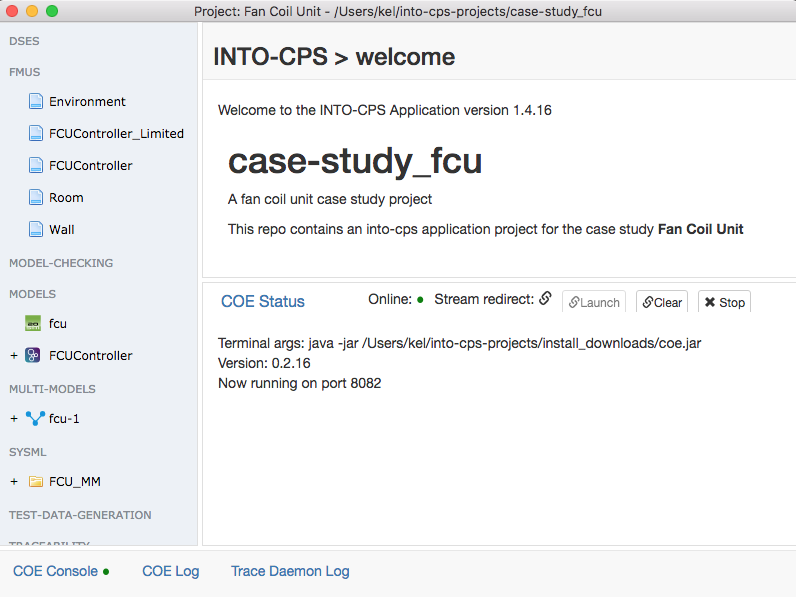
\includegraphics[width=\textwidth]{./figures/app/main}
\caption{\intoapp{} main window.}
\label{fig:app-main}
\end{figure}
%
%
%
\subsection{Projects}
\label{sub:projects}
An \into project contains all the artifacts used and produced by the tool
chain. The project artifacts are grouped into folders. You can create as
many folders as you want and they will all be displayed in the project browser.
The default set of folders for a new project, shown in Figure \ref{fig:app-proj}, is:
%
%
%
\begin{figure}[ht]
\centering
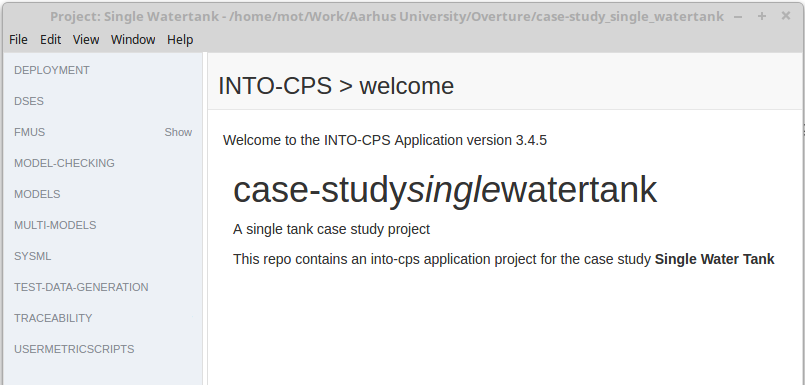
\includegraphics[width=0.85\textwidth]{./figures/app/projbrowser}
\caption{\into project shown in the project browser.}
\label{fig:app-proj}
\end{figure}
%
%
%
\begin{description}
  \item[DSES] Scripts and configuration files for
    performing DSE experiments.
  \item[FMUs] FMUs for the constituent models of the project.
  \item[Model-Checking] Configuration files for performing Model Checking experiments.
  \item[Models] Sources for the  constituent models of the project.
  \item[Multi-Models] The multi-models of the project, using the project FMUs. This
    folder also holds configuration files for performing co-simulations.
  \item[SysML] Sources for the SysML model that defines the architecture and
    connections of the project multi-model. 
  \item[Test-Data-Generation] Configuration files for performing test data
    generation experiments.
  \item[Traceability]  Traceability-specific files plus context menu for traceability information.
  \item[userMetricScripts]  Data analysis scripts.
\end{description}
%
%
%
In order to create a new project, select \textit{File} $\rightarrow$ \textit{New Project}, as shown
in Figure \ref{fig:newproj-menu}. This opens the dialog shown in
Figure \ref{fig:newproj-diag}, where you must choose the project name and location -- the chosen location will be the root of the project, so you should manually
create a new folder for it.
%
%
%
\begin{figure}
  \centering
  \begin{subfigure}[b]{0.45\textwidth}
    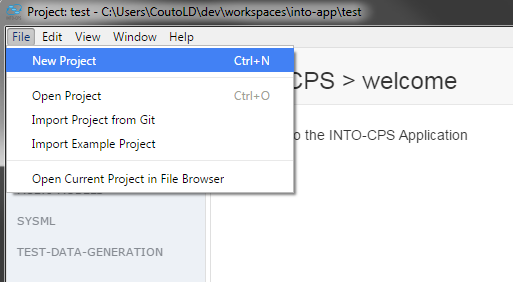
\includegraphics[width=\textwidth]{figures/app/newproj-menu}
    \caption{\emph{New Project} menu entry.}
    \label{fig:newproj-menu}
  \end{subfigure}
  \quad 
  \begin{subfigure}[b]{0.45\textwidth}
    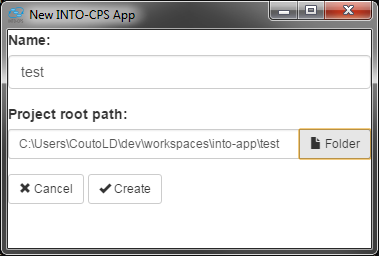
\includegraphics[width=\textwidth]{figures/app/newproj-diag}
    \caption{\emph{New Project} dialog.} 
    \label{fig:newproj-diag}
  \end{subfigure}
  \caption{Creating a new INTO-CPS project.}
  \label{fig:newproj}
\end{figure}
%
%
%
To open an existing project, select \textit{File} $\rightarrow$ \textit{Open Project}, then navigate to the project's root folder and open it. 

To import a project stored in the Git version control system, select
\textit{File} $\rightarrow$ \emph{Import Project from Git}, as shown in Figure \ref{fig:gitproj-menu}.
This opens the dialog shown in Figure \ref{fig:gitproj-diag}, where you must
choose the project location and also provide the Git URL. The project is checked
out using Git, so any valid Git URL will work. You must also have Git available
in your PATH environment variable in order for this feature to work.
%
%
%
\begin{figure}
\centering
\begin{subfigure}[b]{0.45\textwidth}
  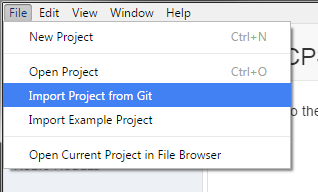
\includegraphics[width=\textwidth]{figures/app/gitproj-menu}
  \caption{\emph{Import Git Project} menu entry.}
  \label{fig:gitproj-menu}
\end{subfigure}
\quad 
\begin{subfigure}[b]{0.45\textwidth}
  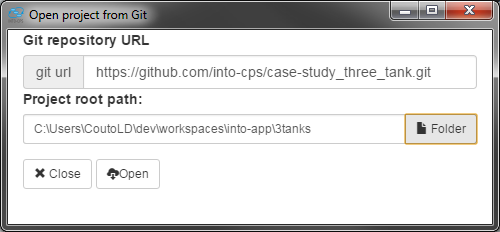
\includegraphics[width=\textwidth]{figures/app/gitproj-diag}
  \caption{\emph{Import Git Project} dialog.} 
  \label{fig:gitproj-diag}
\end{subfigure}
\caption{Importing a Git project.}
\label{fig:gitpro}
\end{figure}
%
%
%
It is possible to import several public example projects that show off
the various features of the \into tool chain. These examples
are described in Deliverable D3.6 \cite{INTOCPSD3.6}. To import an example, select
\textit{File} $\rightarrow$ \emph{Im\-port\ Ex\-amp\-le\ Pro\-ject}, as shown in Figure \ref{fig:example-menu}.
This opens the dialog box shown in Figure \ref{fig:example-diag}, where you 
must select which example to import and a project location. The example
is checked out via Git, so you must have Git available in your path in order
for this feature to work.
%
%
%
\begin{figure}[h!]
\centering
\begin{subfigure}[b]{0.45\textwidth}
  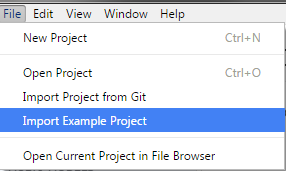
\includegraphics[width=\textwidth]{figures/app/example-menu}
  \caption{\emph{Import Example Project} menu.}
  \label{fig:example-menu}
\end{subfigure}
\quad 
\begin{subfigure}[b]{0.45\textwidth}
  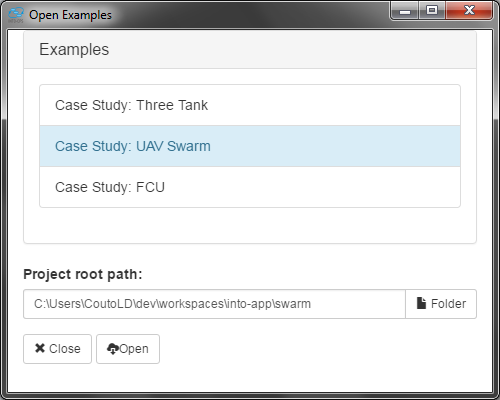
\includegraphics[width=\textwidth]{figures/app/example-diag}
  \caption{\emph{Import Example Project} dialog.} 
  \label{fig:example-diag}
\end{subfigure}
\caption{Importing examples.}
\label{fig:example}
\end{figure}
%
%
%
For both Git projects and examples, once you begin the import process,
a process dialog is displayed, as shown in Figure \ref{fig:git-prog}.

\begin{figure}[ht]
\centering
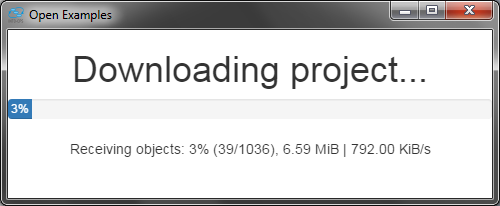
\includegraphics[width=0.45\textwidth]{./figures/app/git-prog}
\caption{Progress of project imports through Git.}
\label{fig:git-prog}
\end{figure}
%
%
%
\subsection{Multi-Models}
\label{sub:multi-models}
For any given project, the \intoapp{} allows you to create and edit multi-models and
co-simulation configurations. To create a new multi-model, right click the
\textit{Multi-models} node in the project browser and select  \textit{New
multi-model}, as shown in Figure \ref{fig:new-mm}. After creation, the new
multi-model is automatically opened for editing.
%
%
%
\begin{figure}[h!]
\centering
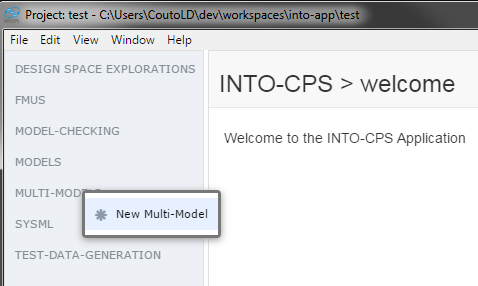
\includegraphics[width=0.65\textwidth]{./figures/app/new-mm}
\caption{Creating a new multi-model.}
\label{fig:new-mm}
\end{figure}
%
%
%
To select an existing multi-model for editing, double-click it. 
Once a multi-model is open, the multi-model view, shown in
Figure \ref{fig:mm-view} is displayed. The top box, \textit{Overview},
displays an overview of the input and output variables in the FMUs,
as shown in Figure \ref{fig:mm-overview}. The bottom box, \textit{Configuration}, enables the user to configure the multi-model.
%
%
%
\begin{figure}[h!]
\centering
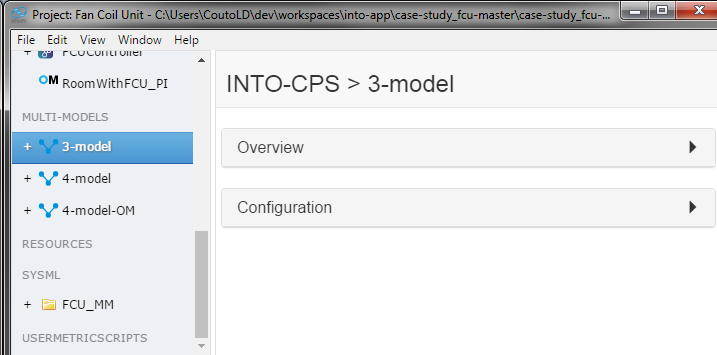
\includegraphics[width=0.75\textwidth]{./figures/app/mm-view}
\caption{Main multi-model view.}
\label{fig:mm-view}
\end{figure}
%
%
%
\begin{figure}[h!]
\centering
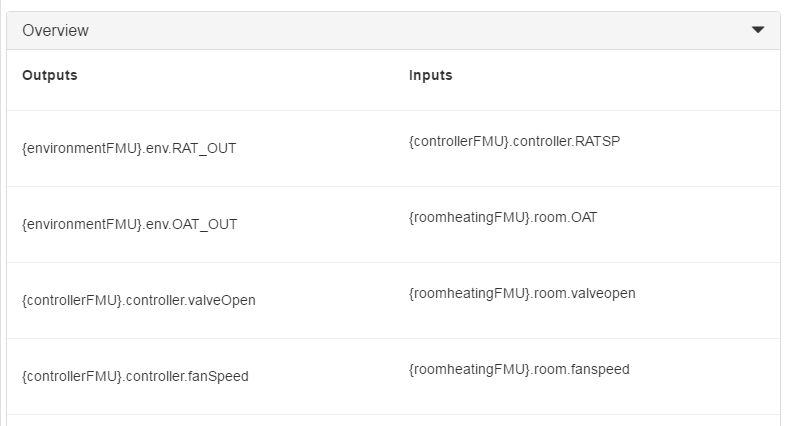
\includegraphics[width=\textwidth]{./figures/app/mm-overview}
\caption{Multi-model overview.}
\label{fig:mm-overview}
\end{figure}
%
%
%
In order to configure a multi-model, it must first be unlocked for editing
by clicking the \textit{Edit} button at the bottom of the \textit{Configuration}
box. There are four main areas dedicated to configuring various aspects of a multi-model.

The \textit{FMUs} area, shown in Figure \ref{fig:mm-fmus}, allows you to remove or add
FMUs and to associate the FMUs with their files by browsing to,
or typing, the path of the FMU file. For each FMU file a marker is
displayed indicating whether the FMU is supported by the \intoapp{} and can be used for co-simulation on the current platform.
%
%
%
\begin{figure}[h!]
\centering
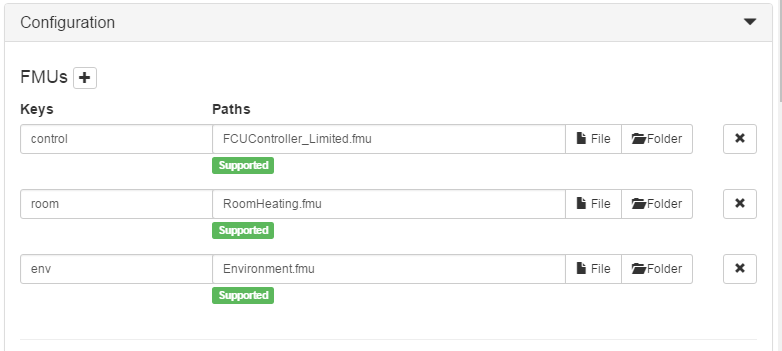
\includegraphics[width=0.9\textwidth]{./figures/app/mm-fmus}
\caption{FMUs configuration.}
\label{fig:mm-fmus}
\end{figure}
%
%
%
The \textit{FMU instances} area, shown in Figure \ref{fig:mm-instances}, allows you to
create or remove FMU instances and name them. A multi-model consists of one or more interconnected instances of various FMUs. More than one instance may be created for a given FMU.
%
%
%
\begin{figure}[h!]
\centering
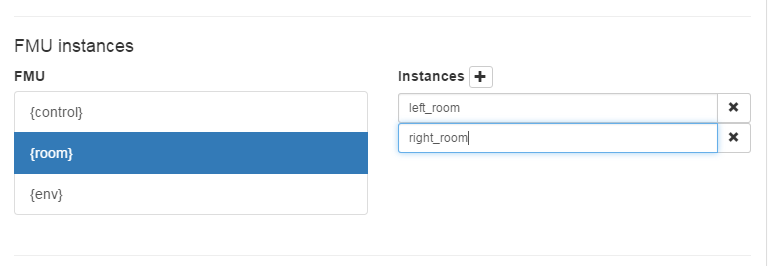
\includegraphics[width=0.9\textwidth]{./figures/app/mm-instances}
\caption{FMU instances configuration.}
\label{fig:mm-instances}
\end{figure}
%
%
%
As a convenient workflow shortcut, the \textit{Connections} area, shown in Figure \ref{fig:mm-conns}, allows you to
connect output variables from an FMU instance into input variables of another:

\begin{enumerate}
  \item Click the desired output FMU instance in the first column.  The output variables for the selected FMU appear in the second column.
  \item Click the desired output variable in the second column.  The input instances appear in the third column.
  \item Click the desired FMU input instance in the third column.  The input variables for the selected FMU appear in the fourth column.
  \item Check the box for the desired input variable in the fourth column.
\end{enumerate}
%
%
%
This facility makes it unnecessary to return to Modelio whenever small changes must be made to the connection topology of the multi-model\footnote{Changes made to a multi-model or FMU outside of the \intoapp{} will cause internal CRC checks to fail.  If this route is taken, it will be necessary to open the multi-model configuration again in the \intoapp{} and go through the edit-save procedure without making any changes.  This will re-validate the multi-model configuration.}.
%
%
%
\begin{figure}[h!]
\centering
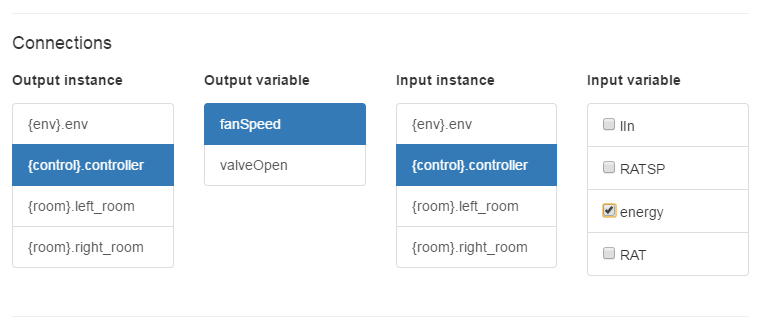
\includegraphics[width=\textwidth]{./figures/app/mm-conns}
\caption{Connections configuration.}
\label{fig:mm-conns}
\end{figure}
%
%
%
The \textit{Initial values of parameters} area, shown in
Figure \ref{fig:mm-params}, allows you to set the initial values of any parameters
defined in the FMUs:
%
%
%
\begin{enumerate}
  \item Click the desired FMU instance in the \textit{Instance Column}.
  \item Select the desired parameter in the \textit{Parameters} dropdown box and click \textit{Add}.
      \item Type the parameter value in the box that appears.
\end{enumerate}
%
%
%
\begin{figure}[ht]
  \centering
  \begin{subfigure}[b]{0.8\textwidth}
    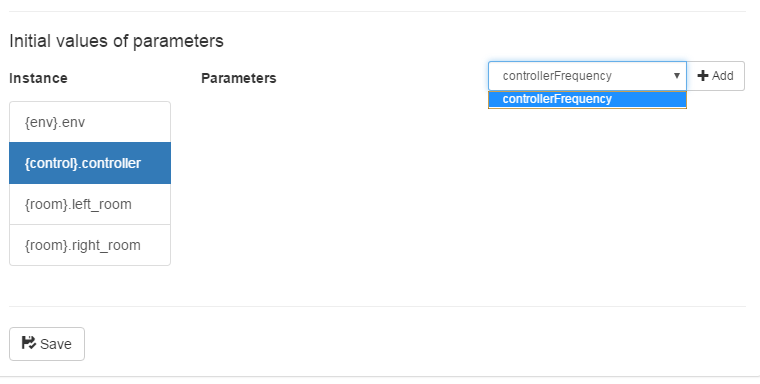
\includegraphics[width=\textwidth]{figures/app/mm-params}
    \caption{Parameter selection.}
    \label{fig:mm-params1}
  \end{subfigure}
  \quad
  \begin{subfigure}[b]{0.8\textwidth}
    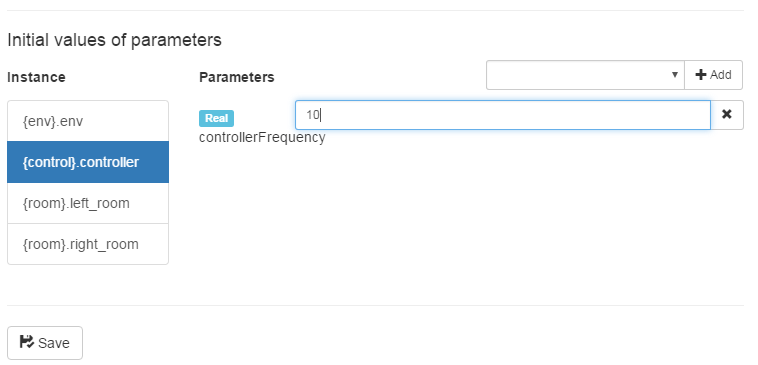
\includegraphics[width=\textwidth]{figures/app/mm-params2}
    \caption{Parameter value input.} 
    \label{fig:mm-params2}
  \end{subfigure}
  \caption{Initial values of parameters configuration.}
  \label{fig:mm-params}
\end{figure}
%
%
%
Once the multi-model configuration is complete, click the \textit{Save}
button at the bottom of the \textit{Configuration} box.
%
\clearpage
%
%
%
\subsection{Co-simulations}
\label{sec:co-simulations}
To execute co-simulations of a multi-model, a co-simulation configuration is
needed. To create a co-simulation configuration, right click the desired
multi-model and select \textit{Create Co-Simulation Configuration}, as shown in Figure \ref{fig:new-cosim}.  After creation, the new configuration automatically opens for editing.
%
%
%
\begin{figure}[ht]
\centering
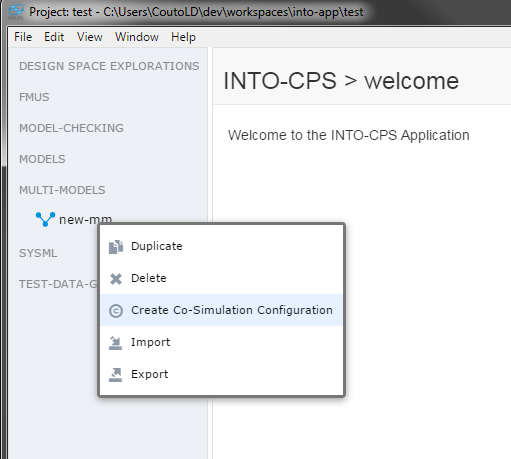
\includegraphics[width=0.7\textwidth]{./figures/app/new-cosim}
\caption{Creating a co-simulation configuration.}
\label{fig:new-cosim}
\end{figure}
%
%
%
To select an existing co-simulation configuration, double-click it. 
Once a configuration is open, the co-simulation configuration, shown in
Figure \ref{fig:cosim-view}, is displayed. The top box, \textit{Configuration},
lets you configure the co-simulation. The bottom box, \textit{Simulation},
lets you execute the co-simulation.
%
%
%
\begin{figure}[ht]
\centering
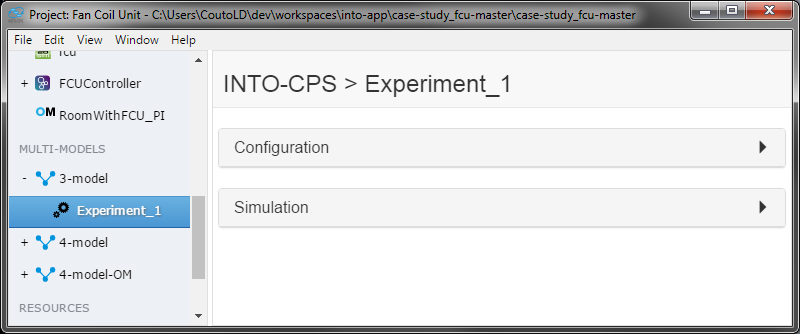
\includegraphics[width=0.8\textwidth]{./figures/app/cosim-view}
\caption{Main co-simulation configuration view.}
\label{fig:cosim-view}
\end{figure}
%
%
%
In order to configure a co-simulation, the configuration must first be unlocked for editing
by clicking the \textit{Edit} button at the bottom of the \textit{Configuration}
box. There are seven things to configure for a co-simulation, discussed next.

\textit{Basic Configuration}, shown in Figure \ref{fig:cosim-top}, allows you to select the start and end time for the co-simulation as well as the master algorithm to be used.
%
%
%
\begin{figure}[ht]
\centering
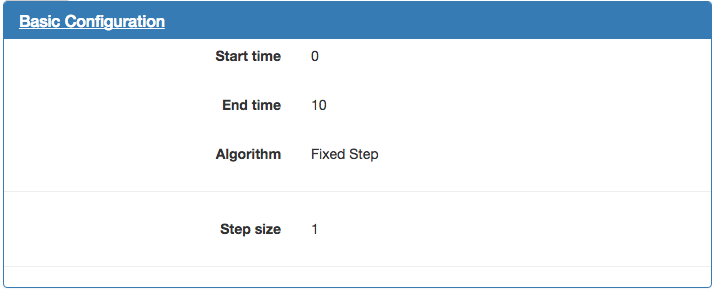
\includegraphics[width=0.8\textwidth]{./figures/app/cosim-top}
\caption{Start/End time and master algorithm configuration.}
\label{fig:cosim-top}
\end{figure}
%
%
%
For every algorithm, there are configuration parameters that can be set. These
are displayed below the top area, as shown in Figure \ref{fig:ma-config}. These parameters differ with the master algorithm chosen.  Parameters are further documented in Deliverable D4.3b \cite{INTOCPSD4.3b}.
%
%
%
\begin{figure}[ht]
\centering
\begin{subfigure}[b]{\textwidth}
  
\includegraphics[width=\textwidth]{figures/app/ma-config-fixed}
  \caption{Fixed step size.}
  \label{fig:ma-conf-fix}
\end{subfigure}
\begin{subfigure}[b]{\textwidth}
  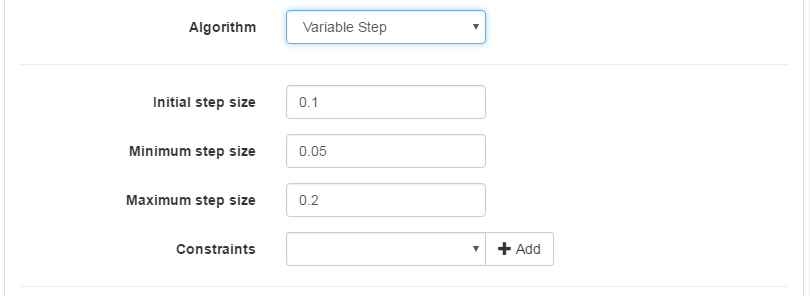
\includegraphics[width=\textwidth]{figures/app/ma-config-variable}
  \caption{Variable step size.}
  \label{fig:ma-conf-var}
\end{subfigure}
\caption{Master algorithm configuration.}
\label{fig:ma-config}
\end{figure}
%
%
%

The \textit{Visibility} area, shown in Figure \ref{fig:visibility-config}, controls loggable FMU output.  \emph{Visible} indicates whether the FMU gives any visible feedback, \emph{e.\@g.\@} graphs.  \emph{Logging on} indicates whether the FMU should use the logging system and send log info back to the COE.  \emph{Enable all log categories per instance} enables all log categories listed inside each FMU.  \emph{Global coe log level override} enables the user to override the pre-set log level in the COE.  This is for debugging failing simulations and should be left unset or at ``error'' or ``warning'' level.
%
%
%
\begin{figure}[ht]
\centering
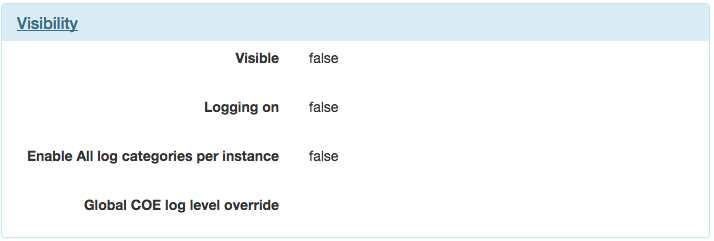
\includegraphics[width=0.9\textwidth]{figures/app/visibility}
\caption{Visibility configuration.}
\label{fig:visibility-config}
\end{figure}
%
%
%

The \emph{Stabilization} area, shown in Figure \ref{fig:stabilization-config}, allows the user to enable the global co-simulation stabilization feature.  These parameters are passed to the NumPy \texttt{isclose()} function\footnote{\url{https://docs.scipy.org/doc/numpy-1.13.0/reference/generated/numpy.isclose.html}}.
%
%
%
\begin{figure}[ht]
\centering
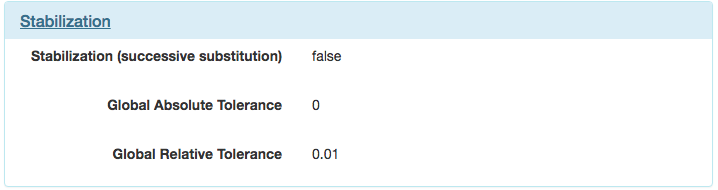
\includegraphics[width=0.9\textwidth]{figures/app/stabilization}
\caption{Stabilization configuration.}
\label{fig:stabilization-config}
\end{figure}
%
%
%

The \textit{Live Plotting} area, shown in Figure \ref{fig:liveplotting-conf}, enables the user to define multiple graphs (currently this comes at a relatively high display cost.)  Each graph can either be external (in its own window) or internal (embedded). The internal graphs are arranged in a configurable grid.  The aim of the grid layout is to eliminate the need for scrolling.  Additional rows are added if no space is left, but these introduce scrolling. When configuring the graphs, it is possible to use a filter on all available scalar variables to find the ones of interest.
%
%
%
\begin{figure}[ht]
\centering
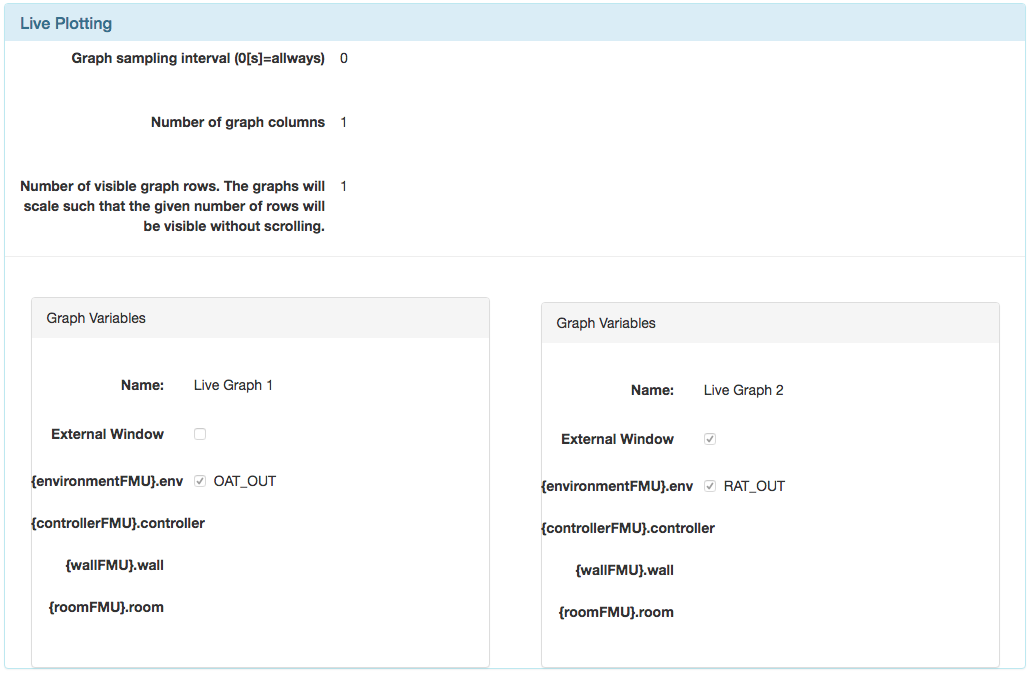
\includegraphics[width=\textwidth]{./figures/app/livePlotting}
\caption{Live plotting configuration.}
\label{fig:liveplotting-conf}
\end{figure}
%
%
%

The \emph{Results Saving} area, shown in Figure \ref{fig:saving-conf}, allows the user to select additional FMU variables to log in the global CSV log file.  All connected variables are logged by default.
%
%
%
\begin{figure}[ht]
\centering
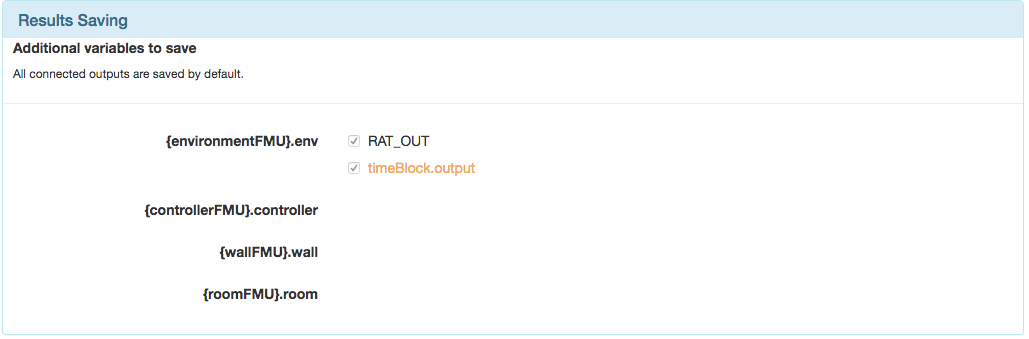
\includegraphics[width=\textwidth]{./figures/app/resultsSaving}
\caption{Results logging configuration.}
\label{fig:saving-conf}
\end{figure}
%
%
%

The \emph{Others} area, shown in Figure \ref{fig:others-conf}, allows the user to slow the co-simulation down to wall time and to enable co-simulation parallelisation.  Please note that parallelising a co-simulation does not always result in a speed-up \cite{Thule&16c}.
%
%
%
\begin{figure}[ht]
\centering
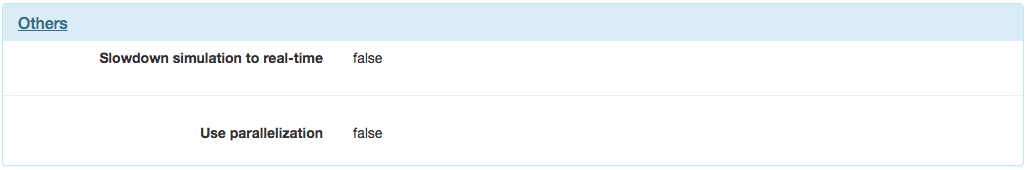
\includegraphics[width=\textwidth]{./figures/app/others}
\caption{Miscellaneous configuration options.}
\label{fig:others-conf}
\end{figure}
%
%
%

The final area, \emph{Post-Processing}, shown in Figure \ref{fig:postprocess}, allows the user to attach a post-processing script written in Python that can be executed at the end of co-simulations.
%
%
%
\begin{figure}[ht]
\centering

\includegraphics[width=\textwidth]{./figures/app/postProcessing}
\caption{Attaching a post-processing script.}
\label{fig:postprocess}
\end{figure}
%
%
%

Once the co-simulation configuration is complete, click the \textit{Save}
button at the bottom of the \textit{Configuration} box.

The \textit{Simulation} box, shown in Figure \ref{fig:cosim-coe}, allows
you to launch a co-simulation. To run a co-simulation, the COE must be
online. The area at the top of the \textit{Simulation} box displays
the status of the COE. If the COE is offline, you may click the
\textit{Launch} button to start it.
%
%
%
\begin{figure}[ht]
\centering
\begin{subfigure}[b]{0.45\textwidth}
  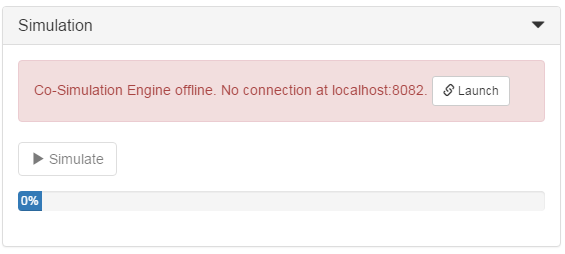
\includegraphics[width=\textwidth]{figures/app/cosim-coe-offline}
  \caption{COE offline.}
  \label{fig:cosim-coe-offline}
\end{subfigure}
\quad 
\begin{subfigure}[b]{0.45\textwidth}
  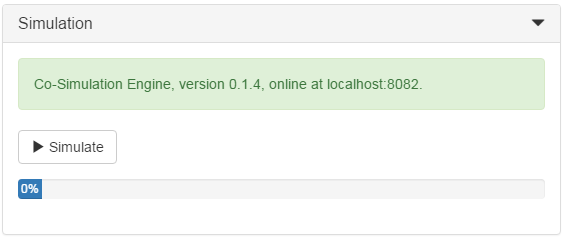
\includegraphics[width=\textwidth]{figures/app/cosim-coe-online}
  \caption{COE online.} 
  \label{fig:cosim-coe-online}
\end{subfigure}
\caption{Launching a co-simulation.}
\label{fig:cosim-coe}
\end{figure}
%
%
%
Once a co-simulation is in progress, any variables chosen for live plotting are plotted in real time in the simulation box, as shown in Figure \ref{fig:cosim-plot}. A progress bar is also displayed.
%
%
%
\begin{figure}[ht]
\centering
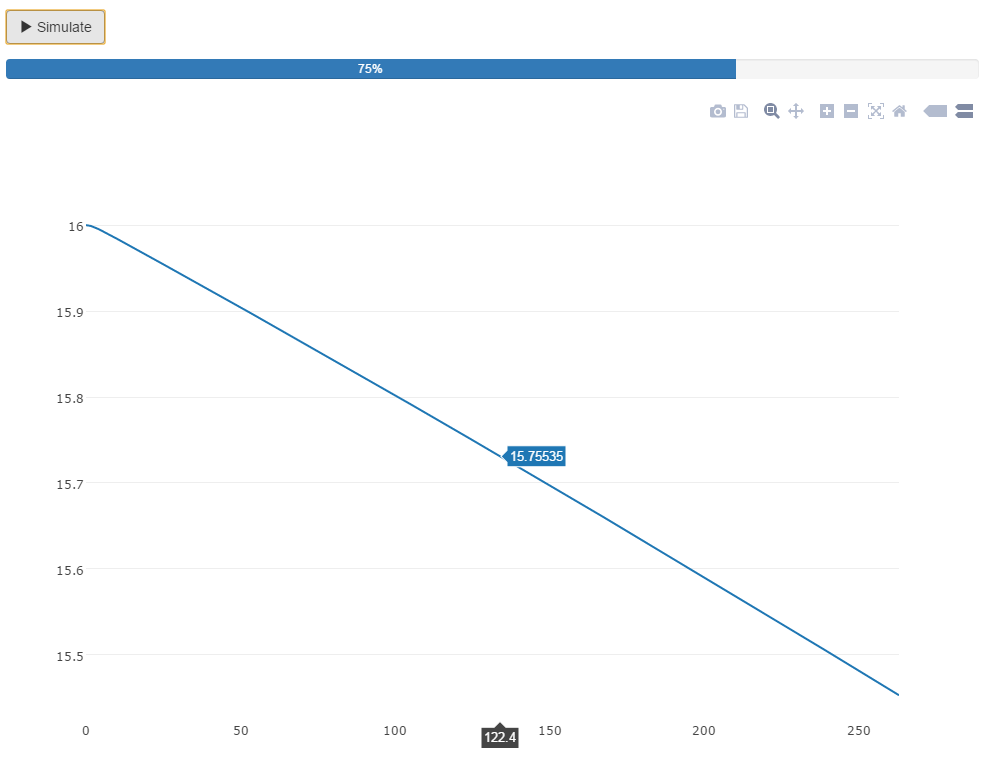
\includegraphics[width=\textwidth]{./figures/app/cosim-plot}
\caption{Live stream variable plot.}
\label{fig:cosim-plot}
\end{figure}
%
%
%
When the simulation is complete, the live stream plot can be explored or
exported as a PNG image. In addition, an \texttt{outputs.csv} file is created
containing the values of every variable marked for logging. This file can be double-clicked and it will open with the
default system program for CSV files. It can also be imported into programs such as R, MATLAB or Excel for more complex analysis. Furthermore, it is possible to add a post-processing script that receives the CSV file name and the total simulation time respectively as arguments. It is also possible to configure the amount of logging performed by the COE.
%
%
%
%\begin{figure}[ht]
%\centering
%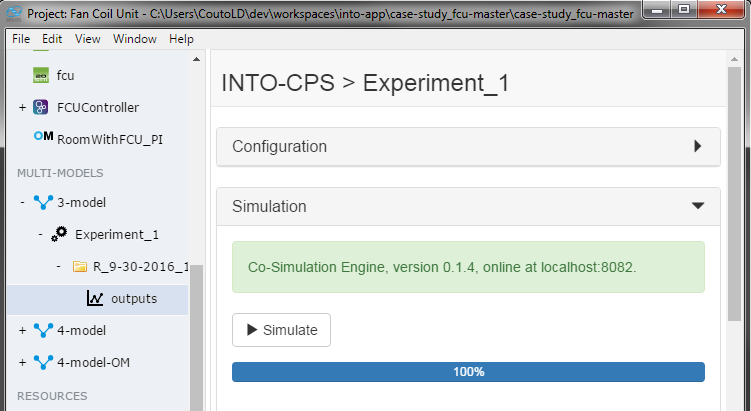
\includegraphics[width=0.85\textwidth]{./figures/app/cosim-results}
%\caption{Co-simulation results file.}
%\label{fig:cosim-results}
%\end{figure}
%
%
%
%\clearpage
%
%
%
\subsection{Additional Features}
\label{sub:other-features}

The \intoapp{} has several secondary features, most of them accessible through
the \textit{Window} menu, as shown in Figure \ref{fig:other-features}. They
are briefly explained below.

\begin{figure}[h!]
\centering
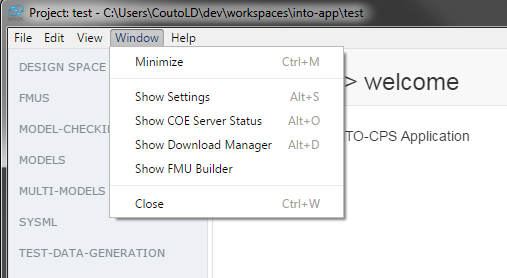
\includegraphics[width=0.65\textwidth]{./figures/app/other-features}
\caption{Additional features.}
\label{fig:other-features}
\end{figure}

\begin{description}
  \item[\texttt{Show Settings}] Displays a settings page where various default
    paths and other options can be set. Development mode can also be enabled from this page, but
    this feature is primarily meant to be used by developers for testing.  Documentation for each setting is found here.
  \item[\texttt{Show Download Manager}] Displays a page where installers can be 
    downloaded for the various tools of the \into tool chain, including the COE.
  \item[\texttt{Show FMU Builder}]  Displays a page that links to a service
    where source code FMUs can be uploaded and cross-compiled for various platforms. Note that this is not a secure service and
    users are discouraged from uploading proprietary FMUs.
\end{description}


\subsection{The Co-Simulation Orchestration Engine}\label{sec:COE}
The heart of the \intoapp{} is the Co-Simulation Orchestration Engine (COE).
%
This is the engine that orchestrates the various simulation tools (described below), carrying out their respective roles in the overall co-simulation.
%
It runs as a stand-alone server hosting the co-simulation API on port 8080.
%
It can be started from the \intoapp{}, but it may be started manually at the command prompt for testing and specialist purposes by executing:
%
%
%
\begin{quote}
\texttt{java -jar coe.jar 8082}
\end{quote}
%
%
%
TCP port 8082 will be chosen by default if it is omitted in the command above.
%
The COE is entirely hidden from the end user of the \intoapp{}, but parts of it are transparently configured through the main interface.
%
The design of the COE is documented in Deliverable D4.1d \cite{INTOCPSD41d}.

The COE is controlled using simple HTTP requests.
%
These are documented in the API manual, which can be obtained directly from the COE by navigating to \url{http://localhost:8082}, once the COE is running.
%
Port 8082 should be changed to that specified when the COE is started.

Following the protocol detailed in the API document, a co-simulation session can be controlled manually from the command prompt using, for example, the \texttt{curl} utility, as demonstrated in the following example.

With the COE running, a session must first be created:
%
%
%
\begin{quote}
\texttt{curl http://localhost:8082/createSession}
\end{quote}
%
%
%
This command will return a \texttt{sessionID} that is used in the following commands.

Next, assuming a COE configuration file called \texttt{coeconf.json} has been created as described in the API manual, the session must be initialized:
%
%
%
\begin{quote}
\texttt{curl -H "Content-Type: application/json" \\ -{}-data @coeconf.json \\ http://localhost:8082/initialize/sessionID}
\end{quote}
%
%
%
Assuming start and end time information has been saved to a file, say \texttt{startend.json}, the co-simulation can now be started:
%
%
%
\begin{quote}
\texttt{curl -H "Content-Type: application/json" \\ -{}-data @startend.json \\ http://localhost:8082/simulate/sessionID}
\end{quote}
%
%
%
Once the co-simulation run ends, the results can be obtained as follows:
%
%
%
\begin{quote}
\texttt{curl -o results.zip \\ http://localhost:8082/result/sessionID/zip}
\end{quote}
%
%
%
The session can now be terminated:
%
%
%
\begin{quote}
\texttt{curl http://localhost:8082/destroy/sessionID}
\end{quote}
%
%
%
The \intoapp{} fundamentally controls the COE in this way.
%
\paragraph{Distributed co-simulations}
Presently the \intoapp{} can only control the COE in this way for non-distributed co-simulations.
%
In order to run a distributed co-si\-mu\-la\-tion, a distributed version of the COE, \texttt{dcoe}, must be controlled from the command prompt manually, as illustrated above.
%
The distributed COE can be downloaded using the App's \emph{Download Manager}.

In a distributed co-simulation the COE and (some) FMUs execute on physically different compute nodes.
%
The FMUs local to the COE computing node are handled in the same way as in standard co-simulations.

Each FMU on the remote nodes is served externally by a daemon process.
%
This process must be started on the remote node manually as follows:
%
%
%
\begin{quote}
\texttt{java -jar daemon*-jar-with-dependencies.jar -host <public-ip> -ip4}
\end{quote}
%
%
%
Here, \texttt{<public-ip>} is the IPv4 address of the compute node.

Next, the distributed COE process must be started manually from the command prompt on its own node, with options specific to distributed co-simulation:
%
%
%
\begin{quote}
\texttt{java -Dcoe.fmu.custom.factory=\\ org.intocps.orchestration.coe.distribution.\\DistributedFmuFactory \\ -jar dcoe*-jar-with-dependencies.jar}
\end{quote}
%
%
%
The second difference is the way in which the location of the remote FMUs is specified.
%
For a standard co-simulation, the \texttt{fmus} clause of the co-simulation configuration file (\texttt{coeconf.json}, in our example) contains elements of the form
%
%
%
\begin{quote}
\texttt{``file://fmu-1-path.fmu''}
\end{quote}
%
%
%
These must be modified for each remote FMU to the following URI scheme:
%
%
%
\begin{quote}
\texttt{``uri://<public-ip>/FMU/\#file://local-fmu-path.fmu''}
\end{quote}
%
%
%
The COE configuration file can, of course, be written manually in its entirety, but it is possible to take a faster route, as follows.

This configuration file is only generated when a co-simulation is executed.
%
It is therefore possible to assemble a ``dummy'' co-simulation that is similar to the desired distributed version, but with a local FMU topology.
%
Since it is likely that the remote FMUs are not supported on the COE platform itself, it is necessary here to construct ``dummy'' FMUs with the same interface.
%
If this local co-simulation is then executed briefly, a COE configuration file will be emitted that can be easily modified as described above.
%
The \intoapp{} will name this file \texttt{config.json} and emit it to the \texttt{Multi-models} folder under each co-simulation run.
%
This modified configuration can then be used to execute the distributed co-simulation.
